% TODO_ The following notions must have been introduced before:
% - The trace invariant (but not the message invariant)

\chapter{Case study}

Now that we have presented our methodology and its implementation in the Reusable Verification Library, we will apply it to a protocol to showcase its use. 
In this chapter, our goal is to show that the library is now able to verify a protocol whose security properties rely on the frequent deletion of sensitive data.

\todo{Write the outline}

\section{Choosing a protocol to verify}
\label{sec:choosing-a-protocol-to-verify}

First, we decide on a protocol to verify.
We take several criteria into account, that we list here in order of importance.
First, the protocol must use ephemeral keys, that exist only for a short time before being deleted, to satisfy some strong security property.
Second, we want the protocol to be simple enough to be implemented and verified in a reasonable amount of time. As we only aim to showcase the use of our extended verification library, there is no need to use a state-of-the-art security protocol.
And third, we want to derive our protocol from an existing one, to show that our library can verify real-world protocols, and not only toy examples.

\todo{Write the outline}

\subsection{Ratcheting protocols}
\label{sec:ratcheting-protocols}
% DH Ratchet, Signal

We have already mentioned the Signal protocol in the previous chapters, which is based on the Double Ratchet algorithm.
Signal is a state-of-the-art protocol, whose verification of a Go implementation has, to the best of our knowledge, never been attempted.
However, we do not consider that we have sufficient time to verify such a complex protocol implementation in the scope of this thesis.
Optimally, we would like to verify a protocol implementation that is simpler than Signal, but uses the same principles of ephemeral keys and ratcheting to achieve comparable security properties.

Such a protocol exists and has already been introduced in section \ref{sec:diffie-hellman-ratchet}: the Diffie-Hellman (DH) Ratchet.
Recall that the DH Ratchet is the core component of the Signal protocol. Participants frequently exchange their Diffie-Hellman public keys and use them to obtain a shared secret that is used to derive new ephemeral keys to encrypt their messages.
The DH Ratchet aims to provide both forward secrecy and post-compromise security, which are the same security properties that Signal aims to achieve.
If the DH Ratchet can provide the same guarantees as the more complex Signal protocol, it is because the DH Ratchet uses a simpler communication model, where participants alternate sending and receiving messages.
In Signal, the protocol has to cope with a participant sending multiple messages in a row, as well as out-of-order and lost messages.

While the DH Ratchet now appears to be a good candidate for our case study, we have to handle the fact that it requires some prior knowledge, as shown in Figure \ref{fig:dh-ratchet}.
We need to provide the initiator and responder with a shared secret $K_0$, which will be the initial key of their key chain.
Additionally, we need to provide the initiator with the public key $g^{y_0}$ of the responder, where $y_0$ is the private of the responder.
We cannot use the DH Ratchet without this prior knowledge, which requires us to add an initial key agreement to the protocol.

\subsection{Initial key agreement}
\label{sec:initial-key-agreement}
% X3DH, WireGuard noise's Handshake

Similarly to the Diffie-Hellman Ratchet, the Signal protocol starts with an initial key agreement before running the Double Ratchet algorithm.
Signal uses the X3DH key agreement protocol, which is a state-of-the-art protocol that provides forward secrecy and cryptographic deniability.
Additionally, X3DH is specifically designed to work asynchronously when one user is offline.
Because X3DH is a complex protocol that would require significant time to implement and verify, and because we do not necessarily need all of its strong security properties, we are going to use a simpler protocol.

We use the fact that the WireGuard protocol has already been implemented and verified with the Reusable Verification Library.
WireGuard starts with a handshake based on a Diffie-Hellman key exchange, called the \emph{Noise\_IK} handshake from the Noise protocol. This handshake establishes symmetric keys between the initiator and responder, which is the first part of the prior knowledge required by the DH Ratchet.
\todo{Should I mention the security properties of the handshake (strong/weak forward secrecy)?}

Then, it is easy to add a communication round between the initiator and responder, in which the responder computes a Diffie-Hellman key pair and sends its public key to the initiator, authenticated with the symmetric key established by the handshake.\todo{This is not really a communication “round” because there is just one message, no response.}
Therefore, if we combine the \emph{Noise\_IK} handshake with this additional communication round, we obtain the prior knowledge required by the DH Ratchet.
At this point, we have a ratcheting protocol that satisfies the three criteria introduced at the beginning of this section. However, we made an additional modification to simplify the verification process.

\subsection{Chosen protocol}
\label{sec:chosen-protocol}

As shown in Figure \ref{fig:dh-ratchet}, when the initiator sends a message encrypted by a key $K_1$ to the responder together with its new public key $g^{x_1}$, the responder uses this public key $g^{x_1}$ to compute the shared secret $K_1$ and decrypt the message.
Typically, the public key $g^{x_1}$ is sent in the associated data of the AEAD encrypted message, so its integrity is protected, but it remains publicly readable so the responder can immediately access it to compute $K_1$.

In the existing methodology and its current implementation, the Reusable Verification Library, the message comes with a ghost \emph{message invariant}. It is a property, part of the trace invariant, about the content of the message used for verification purposes. Upon encrypting the message to send, the initiator has to prove this message invariant, and upon receiving and decrypting the message, the responder can either assume the message invariant or know that corruption has occurred.
In our case, for the first message sent by the initiator on Figure \ref{fig:dh-ratchet}, the message invariant would contain information about the public key $g^{x_1}$. In particular, it would contains that $g^{x_1}$ is an exponential with base generator $g$ and exponent $x_1$, where $x_1$ is a nonce readable by the initiator.
This information can then be used for verification purposes on the responder side, notably to know that $g^{x_1y_0}$ is a Diffie-Hellman shared secret.

However, in our case, it is a problem that the message invariant is obtained only \emph{after} decryption of the message because we would need to know that $g^{x_1y_0}$ is a shared secret \emph{before} decryption to be able to decrypt the message.
Indeed, the decryption function requires us to prove that $K_1$ is a valid AEAD decryption key, which we can only know if we know that $g^{x_1y_0}$ is a shared secret.
\todo{Why don't we obtain the message invariant upon message reception instead of decryption? Could we change the methodology or library to make the DH Ratchet protocol verifiable?}

This is why we decided to slightly modify the DH Ratchet protocol to make it verifiable with our existing methodology and library.
We present our modified protocol in Figure \ref{fig:dh-ratchet-modified}, and our new first communication round (running after the \emph{Noise\_IK} handshake) in Figure \ref{fig:dh-ratchet-modified-first}.
For the sake of readability, we will now refer in all future parts to our modified DH Ratchet protocol as the \emph{ratcheting protocol}. Additionally, we will refer to the full protocol that we verify, e.g. the \emph{Noise\_IK} handshake followed by the first communication round and the ratcheting protocol, as the \emph{full protocol}.

\begin{figure}
    \centering
    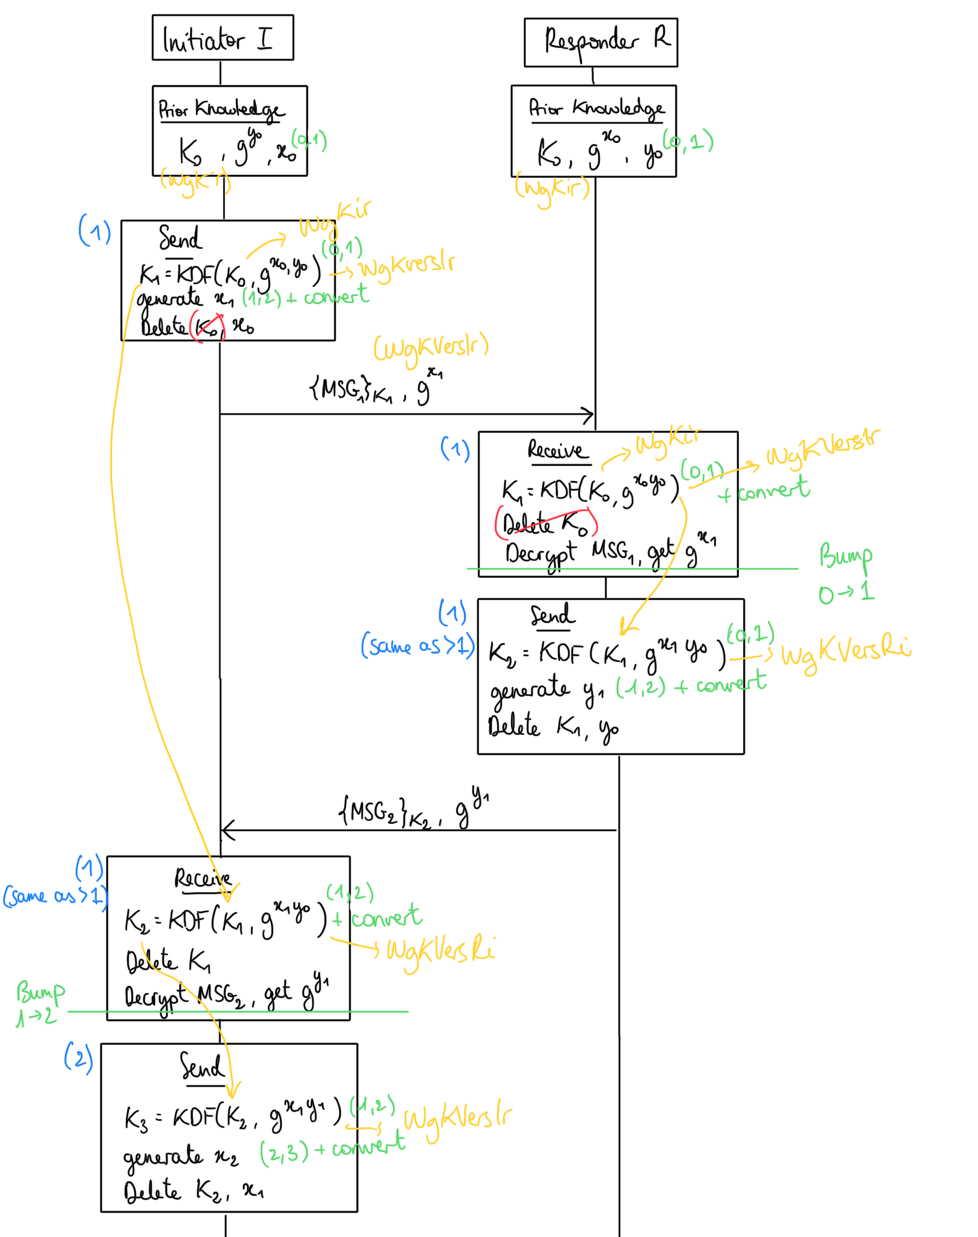
\includegraphics[width=0.9\textwidth]{figures/DH-ratchet-modified.png}
    \caption{Diffie-Hellman Ratchet protocol.}
    \label{fig:dh-ratchet-modified}
\end{figure}

\begin{figure}
    \centering
    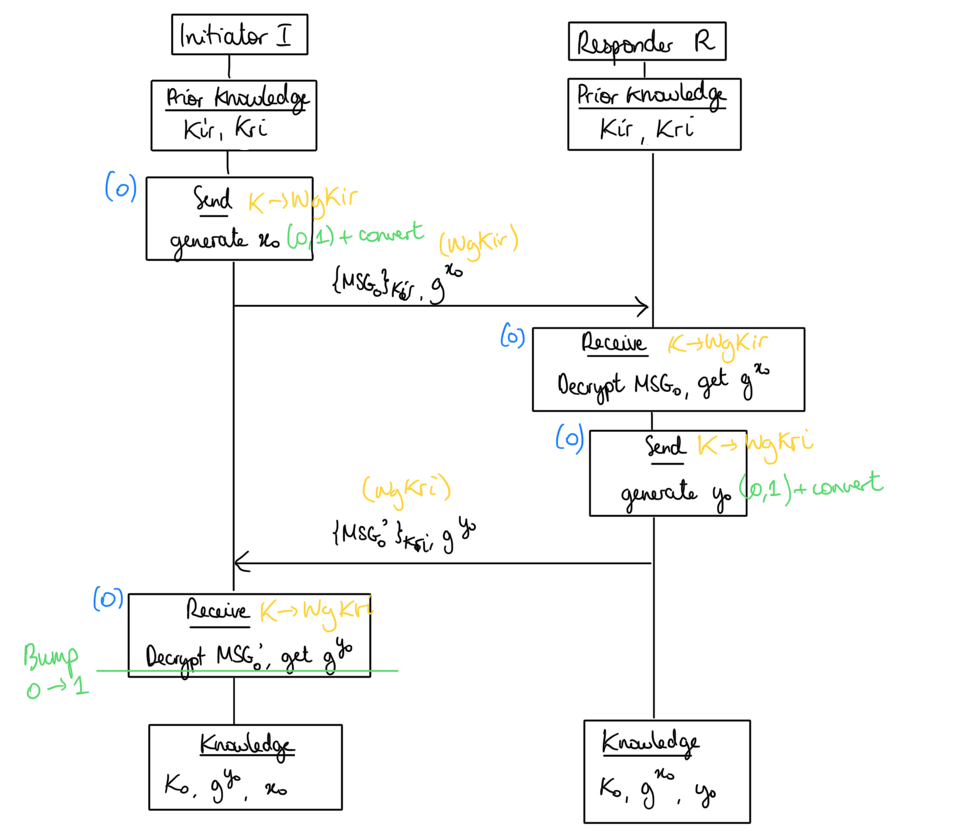
\includegraphics[width=0.9\textwidth]{figures/DH-ratchet-modified-first.png}
    \caption{Diffie-Hellman Ratchet protocol.}
    \label{fig:dh-ratchet-modified-first}
\end{figure}
\todo{Change the figures \ref{fig:dh-ratchet-modified} and \ref{fig:dh-ratchet-modified-first} to use cleaner ones, and modify the caption to explain the figures more in detail}

The intuition behind the ratcheting protocol is that we replicate the DH Ratchet protocol, but instead of using the just received public key to compute the shared secret used in the message decryption, we use the public key received in the previous message.
This first requires us to modify the prior knowledge of the participants. Now, in addition to the initial shared secret $K_0$, both participants need to know the other's public key and their private key.
This is the purpose of the new first communication round shown in Figure \ref{fig:dh-ratchet-modified-first}. 
Like before, the initiator sends its public key $g^{x_0}$ to the responder, authenticated with the symmetric key established by the handshake. But then, the responder replies with its authenticated public key $g^{y_0}$.

Coming back to the ratcheting protocol shown in Figure \ref{fig:dh-ratchet-modified}, when computing the first shared secret $K_1$, the initiator uses its private key $x_0$, whose associated public key $g^{x_0}$ is already known by the responder, from the first communication round.
This was not the case in the DH Ratchet protocol.
The first message sent by the initiator to the responder is otherwise the same as in the DH Ratchet protocol and contains the initiator's new authenticated public key $g^{x_1}$ in addition to the encrypted message.
Upon reception of this message by the responder, instead of using the public key $g^{x_1}$ to compute the shared secret $K_1$, the responder uses the previous public key $g^{x_0}$ received in the first communication round.
This allows the responder to obtain $K_1$, decrypt the message, and obtain the associated message invariant containing information about the new public key $g^{x_1}$.
Then, $g^{x_1}$ is used just after by the responder to compute the next shared secret $K_2$, which is used to encrypt the next message sent to the initiator.
The same observations can be made upon reception of the second message by the initiator, and all subsequent messages. 
\todo{Depending on how precise the final Figure \ref{fig:dh-ratchet-modified} is, I may need to explain the difference between the first message and the others: we do not delete the unversioned key $K_0$}

Ultimately, this ratcheting protocol is simpler to verify than the DH Ratchet and aims to provide similar security properties.
Intuitively, forward secrecy still holds because past communication keys are deleted and cryptographically not retrievable from long-term secrets and current communication keys.

Additionally, post-compromise security still holds but with a stronger assumption.
Recall that post-compromise security \emph{via state} considers that some secret data remains known only by the participants after a compromise.
With the DH Ratchet protocol, we assumed that the attacker compromised Alice's $K_n$ key (and state) \emph{after} she derived $K_{n+1}$, and this assumption was enough to obtain post-compromise security (section \ref{sec:security-properties}).
However, this does not hold in this case.
Suppose we have two participants Alice and Bob communicating, and that an attacker compromises Alice's state at the time when she computed $K_n$ after receiving a message.
The attacker knows $K_n$, but also Alice's ephemeral private key $x_{n-1}$ and Bob's just-received public key $g^{y_{n-1}}$.
The attacker can therefore compute $K_{n+1} = \text{KDF}(K_n, g^{x_{n-1}y_{n-1}})$ because it knows all the inputs of the KDF function, which was not the case with the DH Ratchet protocol.
Unlike before, we have to assume that the attacker compromised Alice's $K_n$ key (and state) after she derived $K_{n+1}$ \emph{and} $K_{n+2}$.
At this point, the attacker cannot obtain $K_{n+2}$ because they cannot have access to the new Diffie-Hellman shared secret.
The protocol is therefore healed and achieves post-compromise security.

In the end, we have presented a full protocol that draws its security properties from the frequent renewal of ephemeral keys. This protocol is mainly based on the Diffie-Hellman Ratchet protocol and has been slightly adapted to facilitate its verification. 
We will now present how we implemented and verified this protocol using our methodology and its implementation in the Reusable Verification Library. 

\section{Implementation and verification}
\label{sec:implementation-and-verification}

\section{Evaluation}
\label{sec:evaluation}